%Included for Gather Purpose only:
%input "MP2P_MacQuire_A.bib"
\documentclass[times, 10pt,twocolumn]{article}
\usepackage{latex8}
\usepackage{times}
\usepackage{epsfig}

\pagestyle{empty}

\begin{document}

\title{Performance Analysis of Stealth DHT with Mobile Nodes}

\author{Andrew MacQuire \quad Andrew Brampton \quad Idris A. Rai \quad Laurent Mathy\\
Computing Department\\Lancaster University\\
\{macquire,brampton,rai,laurent\}@comp.lancs.ac.uk}

\maketitle \thispagestyle{empty}

\begin{abstract}
The advances in wireless networking and the consequent emergence of
new applications that wireless networks increasingly support
inevitably leads to low capability mobile nodes connecting to
peer-to-peer networks.  However, the characteristics of mobile nodes
and limitations of access point coverage often cause mobile nodes to
lose connectivity, which can cause many mobile nodes to
simultaneously leave the network. Continuous departures and joins
due to the mobility of nodes leads to {\em mobility churn}, which
can often degrade the performance of the underlying peer-to-peer
network significantly. In this paper, we use simulations to
demonstrate that the Stealth Distributed Hash Table (Stealth DHT)
algorithm is ideally suited for networks with mobile nodes. By
avoiding storing state in unreliable nodes, a Stealth DHT prevents
mobile nodes from being used by other nodes to provide services.
Consequently, Stealth DHTs eliminate the mobility churn effect and
significantly reduce the amount of overhead as compared to a generic
DHT.
\end{abstract}

\Section{Introduction} \label{sect-intro}

Previously proposed Distributed Hash Table (DHT)
algorithms~\cite{can01}\cite{pastry01}\cite{chord01} have commonly
assumed connecting an overlay of {\em autonomous} and {\em
homogeneous} nodes together. The autonomicity arises in the sense
that nodes may join or leave the network at any time, as well as
request and provide data as they wish. The homogeneity arises from the
fact that devices on the network are assumed to have similar
capabilities in terms of processing power, storage space and network
access.

%Advances in wireless technologies have, however, resulted in an
%exponential surge in the number of Internet connected mobile devices
%of varying capabilities. Given the recent rise in popularity of
%peer-to-peer applications, it is inevitable that users are highly
%likely to connect these heterogeneous devices to such
%networks~\cite{sgg02}. Compared to fixed nodes, however, mobile
%nodes have a number of limitations that make them inherently
%unreliable to support DHT operations such as putting/getting and
%relaying messages, and that can directly affect the performance of
%the underlying DHT.

Mobile devices, however, are likely to be heterogeneous. They are
also often battery powered and prone to moving in and out of signal
range, both of which commonly cause loss of network connectivity. In
a DHT, it is often the case that a mobile node migrating between
access points has to rejoin, as both its own state about other nodes
and their state about it may have been invalidated. This causes what
is termed {\em mobility churn}~\cite{mobilechurn}. Mobility churn,
just like normal churn~\cite{churn1}, is caused when nodes in a
peer-to-peer network continually join and leave in an unpredictable
fashion. This results is more traffic on the DHT due to churned nodes %both don't redo the join proc
repeating the join procedure, and stale state information having to
be detected and discarded by existing nodes. Unfortunately, this
degrades routing efficiency and increases end to end delay. Many DHT
systems have been shown to simply break down under high levels of
churn~\cite{dhtcomparison}\cite{churn1}. To make matters worse, it
has been shown that severe levels of churn are likely for
peer-to-peer networks with mobile
nodes~\cite{mobilechurn}\cite{dhtmanet01}.

Mobile devices  are also likely to have slow network connections
relative to stationary devices. The GSM standard, for example, is
limited to only 14.4 kbps data transfer. GPRS offers some
improvement, averaging at around 40 kbps as empirically detected
by~\cite{mobilep2p3}. Even with newer third generation (3G) devices,
transfer rates are still likely to be far lower than many wired
devices. In the case of such low bandwidth networks, there is the
danger of DHT signalling consuming all the available bandwidth, thus
blocking user traffic.

We believe that the Stealth DHT algorithm proposed
in~\cite{stealth1} is an elegant solution which adapts existing DHT
algorithms themselves to help resolve these problems.

%While some of the discussed issues regarding the impact of mobile
%nodes on DHTs have been addressed before, we believe that the
%Stealth DHT algorithm proposed in~\cite{stealth1} is an elegant
%solution which adapts existing DHT algorithms themselves to resolve
%these problems. The goal of this paper is to assert this belief by
%using simulations to evaluate the performance of a Stealth DHT in
%mobile environments.

A Stealth DHT is a distributed hash table that addresses the problem
of heterogeneous capabilities by maintaining two distinct sets of
nodes on the network. One set, referred to as {\em stealth nodes},
are made effectively ``invisible'' to all routing operations,
meaning that they will never receive any queries, be requested to
forward messages, or asked to store keys. Consequently, they cannot
intercept nor reply maliciously to any messages on the DHT. Ideally,
less capable nodes on the network should be designated as stealth
nodes, as their lack of responsibilities means they have little
effect upon overall routing performance. The remaining set of nodes
on a Stealth DHT are called {\em service nodes}, which can execute
all the operations supported in a generic DHT. For optimal
performance, service nodes should be more stable and capable than
the stealth nodes, thus can be relied upon for supporting the
network. %AB-Now sure I like the change here

The Stealth DHT algorithm was initially proposed with the aim of
returning control of the peer-to-peer network to its operator,
circumventing the numerous security problems and Digital Rights
Management issues commonly associated with such overlays. Service
nodes are therefore assumed to be owned by a service provider,
which, in addition to their high capabilities, should mean that they
are also trustworthy. Conversely, stealth nodes would be autonomous
devices owned by end-users, who request service(s) from the
provider. In this paper, we examine the case of a service provider
offering service to wireless users only, some of whom are mobile,
while others are stationary.

%AB-This was the start of the previous paragraph
We purposefully breaks the pure peer-to-peer paradigm of treating
all nodes as equal. We believe that it is this assumption that
causes generic DHTs to perform poorly in a mobile environment,
further hindering the development of DHT-based mobile applications.
By excluding less capable nodes from routing decisions via the
stealth node concept and designating the most capable nodes as
service nodes, Stealth DHTs help to eliminate the performance
problems associated with mobility and DHTs. Since state information
regarding the mobile nodes in Stealth DHTs is never recorded, they
will not have any responsibility in the network. Thus, they may
join, leave, and request services at will with relatively little
impact on the performance of the underlying DHT. Better still, if a
service provider owns and manages the service nodes, they will have
a complete control over the provided service. We therefore argue
that a Stealth DHT in mobile environments combines the scalability,
resilience and self-organization of existing DHT based networks with
the greater performance and control of a content distribution
network (CDN).

The rest of this paper is organized as follows. In
section~\ref{sect-overview}, we discuss a brief overview of the
Stealth DHT algorithm. We then consider Stealth DHTs with mobile
nodes in section~\ref{sect-mobile}. We present simulation results
and analyze the performance of a Stealth DHT in comparison with
Pastry (a generic DHT) in section~\ref{sect-eval}.
%In section~\ref{sect-related} we discuss related work.
Finally section~\ref{conclusion} concludes the paper.

\Section{Overview of Stealth DHT} \label{sect-overview}

As discussed in~\cite{stealth1} we have extended a generic DHT
algorithm to allow for two types of nodes in a the DHT, namely {\em
service nodes} and {\em stealth nodes}. Service nodes can execute
all operations supported by generic DHTs, whereas stealth nodes are
prevented from storing keys and forwarding messages. While it is
recommended that the stealth node population be comprised of less
capable nodes, the assignment of role (service or stealth) to nodes
is application dependent and in no way prescribed or constrained by
the Stealth DHT itself.

It is important to note that the routing tables of all nodes in a
Stealth DHT consist exclusively of entries for service nodes.
Consequently, a given node of any type may only send a message to a
service node, which will forward it via other service nodes to its
destination (also a service node). This means that stealth nodes are
incapable of communicating directly with one another, and that
service nodes may only communicate with stealth nodes to reply to a
direct request. Accordingly, stealth nodes cannot normally detect
one another, and when ``quiet'', their presence is invisible to even
the service nodes.

In order to achieve the distinction between a service and a stealth
node, stealth nodes employ a lightweight join mechanism. Unlike
service nodes, they do not complete the classical DHT join procedure
by sending announcement messages, thus keeping them from appearing
in other nodes' routing tables. Correspondingly, when a stealth node
joins the network, no updates are required to routing state, nor
does any state become stale upon such a node leaving the network.

A side effect of this procedure is that stealth nodes do not receive
routing updates, as no other node knows to update them. Over time, a
stealth node therefore has an increasingly stale routing table. To
counteract this problem, a stealth node may attempt to obtain
additional state periodically from the network, either in an active
or passive fashion.

An evaluation of Stealth DHTs for wired networks revealed that
regardless of churn, Stealth DHTs outperform Pastry, a generic DHT,
in many standard DHT measurements such as the average hop count,
relative delay penalty (often referred to as stretch), join overhead
and efficiency of load balancing~\cite{stealth1}. We also found that
in a Stealth DHT increasing the number of stealth nodes had no
significant impact on these metrics. This paper extends the
investigation of Stealth DHT performance to mobile environments. For
a more detailed explanation of the Stealth DHT protocol the curious
reader is referred to our previous work~\cite{stealth1}. %reword?

\Section{Stealth DHTs with mobile nodes} \label{sect-mobile}

In this paper we propose using a Stealth DHT in environments where
fixed network infrastructure and mobile nodes are interconnected. We
assume that a mobile node can simply connect to the system via a
nearby wireless access point or base station. When mobile nodes move
they may receive a new network address upon connection to a new
access point, or they may use an available Mobile IP~\cite{rfc3344}
infrastructure to retain their existing IP address. In the former
case, a node would have to inform the DHT of its address change,
thus inducing mobility churn. In the latter case a node may
temporarily lose connectivity, but references to its IP address in
the DHT will not require updating. A node that retains its IP
address may, however, find that the proximity data it stores locally
has be rendered incorrect. We also assume that a node does not have
any prior knowledge of its mobility pattern, and thus cannot inform
other DHT nodes of any movement or loss of connectivity in advance.

We focus on the case of a peer-to-peer network that offers service
to wireless end-users only. The assumption is made that the
provider's network consists of a number of servers which form the
service node infrastructure for the Stealth DHT overlay. These
service nodes may be installed at strategic locations such as within
close proximity of an existing mobile provider's base station, or
they may be located arbitrarily. On the other hand, the stealth
nodes are made up of end-users' wireless devices, such as mobile
telephones, PDAs, laptops and so on.
%Figure~\ref{fig:mob} illustrates this architecture.

%\begin{figure}[htb]
%\centering \epsfig{file= Mobile.eps, width=0.42\textwidth}
%\caption{A possible fixed service node infrastructure, with
%heterogeneous wireless stealth nodes accessing the DHT via base
%stations and wireless access points} \label{fig:mob}
%\end{figure}

%A mobile node joins the network as a stealth node using the
%lightweight procedure outlined in section~\ref{sect-overview}. Upon
%completion of the join procedure, a connected mobile node may
%consult the routing table it has built in order to determine the
%first hop for a given message on the DHT. The service nodes can then
%route the message amongst themselves, with the eventual destination
%replying to the request directly via the IP infrastructure.

%For example: In Figure~\ref{fig:mob} a mobile node {\bf M} sends a
%DHT {\bf get} message to a service node {\bf S$_1$} via a nearby
%base station {\bf B}. {\bf S$_1$} then forwards the message towards
%its eventual destination {\bf S$_2$} over the DHT. Finally, the
%service node {\bf S$_2$} uses the IP address of the mobile node {\bf
%M} to deliver the {\bf getreply} message directly (shown as a dotted
%line). Note that the {\bf getreply} passing through the base station
%{\bf B} should not be misunderstood as it being routed over the DHT.
%The message has to pass through the base station  only because the
%base station is the wireless access point of the mobile node. It is
%also important to note that {\bf S$_1$} would not necessarily be
%{\bf M}'s selected first DHT hop as shown on the diagram; the case
%may exist that {\bf M} would know about {\bf S$_2$} itself, and be
%able to send its {\bf get} message directly to {\bf S$_2$} through
%base station {\bf B} on the IP infrastructure.

We believe that Stealth DHTs offer an elegant solution to the
performance problems caused by mobile nodes in a twofold manner; by
ensuring mobile nodes are not used as routing intermediaries, and by
removing the need for service nodes to maintain state information
about mobile nodes. We show in the next section that Stealth DHTs
help in preventing stale state information in the peer-to-peer
network due to the mobility of nodes, reducing signalling overhead,
and improving routing efficiency.

\Section{Performance Evaluation} \label{sect-eval}

We extended the support for both Pastry and our Stealth DHT in our
own discrete-event packet-level simulator~\cite{stealth1} to cater
for wireless networks. The underlying network upon which the
simulations were run consisted of 1,000 routers in a transit-stub
configuration with 4\% transit nodes, generated with
GT-ITM~\cite{gtitm}. Each stub/edge router was also designated as a
wireless access point. Nodes were attached to the physical network
in a random fashion, with wireless nodes being attached to the edge
routers via a 1 Mbps shared wireless links, while wired nodes were
connected via their own 1 Mbps link. The wireless nodes had a
average latency of 200 ms while wired nodes had only 5 ms.

%It should also be noted that in all cases, our simulations begin
%with the majority of nodes already connected, so the effects of
%initializing the DHT do not skew any of our results (as numerous
%messages are generated when many nodes join simultaneously).

Randomly selected nodes performed \emph{put} operations for a set of
1,000,000 keys before the simulation. Once the simulation started 10
\emph{get} operations were performed by each node at exponentially
distributed intervals with a mean of six minutes. Keys are requested
following a Zipf distribution with an $\alpha$ parameter of 1.2,
thus providing a realistic access and popularity function as
commonly observed in peer-to-peer networks~\cite{zipf}.

We used a mobility model known as the random waypoint
model~\cite{johnson96dynamic} with ``thinking times'' provided by an
exponential distribution around a 60 minute mean (as observed
in~\cite{kotz:campus}) to model mobility patterns of mobile nodes.
We are aware of existing infrastructure that allow mobile nodes to
preserve their IP addresses when their mobility leads them to change
access points. This, however, does not lead to mobility churn nor
does it lead to stale state information on the network (assuming
they do not move out of signal range entirely). Our interest lies in
demonstrating the benefits that a Stealth DHT will have under
mobility churn in comparison with Pastry. Thus, we simulate Stealth
and Pastry DHTs and compare their performances for the case when,
upon changing their access points, mobile nodes also change their IP
addresses. This scenario is perhaps more realistic due to the
relative lack of deployment of mechanisms such as Mobile IP.

We consider a peer-to-peer network with a fixed number of 1,000
nodes. For the Stealth DHT simulations, we designate 99\% of the
nodes as stealth nodes and the remaining 1\% are designated as
service nodes. To show the impact of mobility on the performance of
the DHTs, the number of mobile nodes in the network is increased
from zero, where all stealth nodes on the network are stationary, to
990 nodes where all stealth nodes are mobile. Service nodes retain
wired connectivity in all of these simulations. For Pastry, 1\% of
nodes correspondingly remain wired and the remaining 99\% of
wireless nodes are changed from all stationary towards all mobile.

Throughout this section we refer to {\em moving} and {\em static}
DHTs, which are distinguished by the fact that in the former case,
wireless nodes are in fact mobile, whereas in the latter, wireless
nodes remain stationary. Stationary wireless nodes do not change
access points and thus they do not lose connectivity as with mobile
nodes. Yet, they suffer from high latency links which they have to
share, unlike wired nodes.

%We next present the simulation results that compare  the impact of
%mobility on message overhead and lookup latency for Stealth DHTs and
%Pastry.

\SubSection{Total number of messages}

\begin{figure}[tbp]
\centering 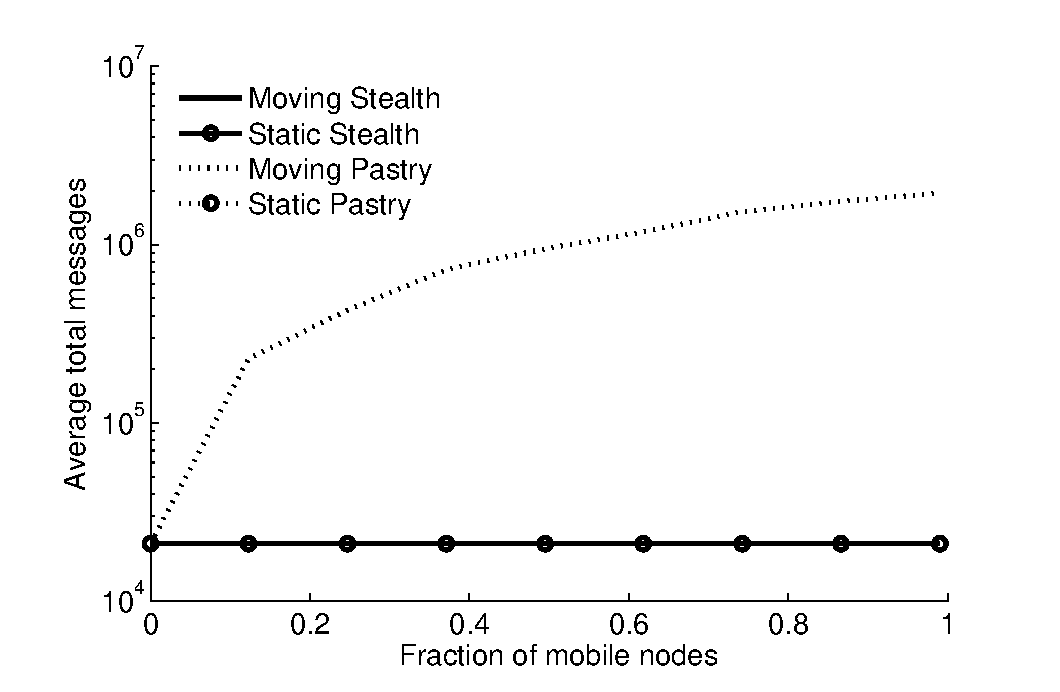
\epsfig{file= messagecount.eps, width=0.42\textwidth}
\caption{Average total no. of messages} \label{fig:msg}
\end{figure}

We first present the results pertaining to the overhead incurred as
a result of node mobility. Figure~\ref{fig:msg} shows the mean total
number of exchanged messages on the DHT, inclusive of {\em put},
{\em get}, {\em getreply} and routing state update messages. The
results are displayed for both moving and static Pastry and Stealth
DHTs as a function of the increase in the fraction of mobile nodes.
We observe that the total number of messages in the Stealth DHT is
constant at 21,000 messages, which indicates that mobility does not
lead to DHT overhead on the network. The figure indicates the same
for both static and moving Stealth DHTs, as well as static Pastry.
This is to be expected, as in these three cases the nodes which are
maintaining state about one another are stationary, meaning they do
not change IP address and thus do not need to update one another.

In contrast, mobility has a severe impact on Pastry.
Figure~\ref{fig:msg} shows that the total number of messages under
moving Pastry is very high and increases with the number of mobile
nodes. The figure illustrates how mobility can lead to many more
messages on the network due to maintenance overhead, as one might
expect.

%When comparing these values it is important to note that we are
%simulating using a slightly optimized version of Pastry, wherein
%nodes may retain their ID and routing state following an IP address
%change. This means that the number of messages are greatly reduced
%as a node need only re-announce its presence upon reconnection;
%there is no need for it to gather routing state again. We believe
%that if we were to simulate with nodes performing a full rejoin, it
%would only serve to increase the gap between the performance of
%Pastry and Stealth DHTs, as the Stealth DHT algorithm was shown to
%significantly reduce the number of messages generated to join a node
%to the network~\cite{stealth1}.

\begin{figure}[tbp]
\centering \epsfig{file= resentcount.eps, width=0.42\textwidth}
\caption{Average no. of resent messages} \label{fig:rsnt}
\end{figure}

\SubSection{Resent messages}

%We assume that a node does not know its mobility pattern in advance.
%Thus, it cannot notify other nodes about its movements, which could
%otherwise help other nodes on the network by removing its state
%information from their routing tables. This avoids forwarding
%messages through a moved node. Instead, when a node changes its
%access point, nodes on the network may erroneously use the state
%information they have retained about it in their attempts to deliver
%messages. If the intended node, whether an intermediate node or the
%final destination, is not available, the message is resent until it
%reaches the existing node with the closest ID in the DHT.

Figure~\ref{fig:rsnt} shows the average number of resent DHT
messages as a function of the increase in the fraction of mobile
nodes in the network. A message is resent whenever a node on the
routing path fails to receive it due to churn. The figure shows the
results for moving Pastry only, as no messages were ever resent
under static Pastry or Stealth DHTs. We observe from the figure the
number of resent messages on the moving Pastry increases rapidly
with an increase in mobile nodes.

The existence of resent messages due to node mobility on a DHT
reflects the unavailability of numerous nodes throughout the
simulation. Thus, resent messages lead to reduced performance in
terms of lookup latency, which we discuss in a later section.

\SubSection{Packets to unreachable hosts}

When a node sends a {\em get} message over the DHT, the recipient
will customarily reply directly to them via the source IP address
contained within the request. While this avoids burdening the DHT
overlay with unnecessary traffic, it also means that {\em getreply}
messages are not counted in Figure~\ref{fig:rsnt}, which refers
solely to messages sent over the DHT.

\begin{figure}[tbp]
\centering \epsfig{file=unreachable.eps, width=0.42\textwidth}
\caption{Average no. of packets sent to unreachable hosts}
\label{fig:unreach}
\end{figure}

\begin{figure}[tbp]
\centering 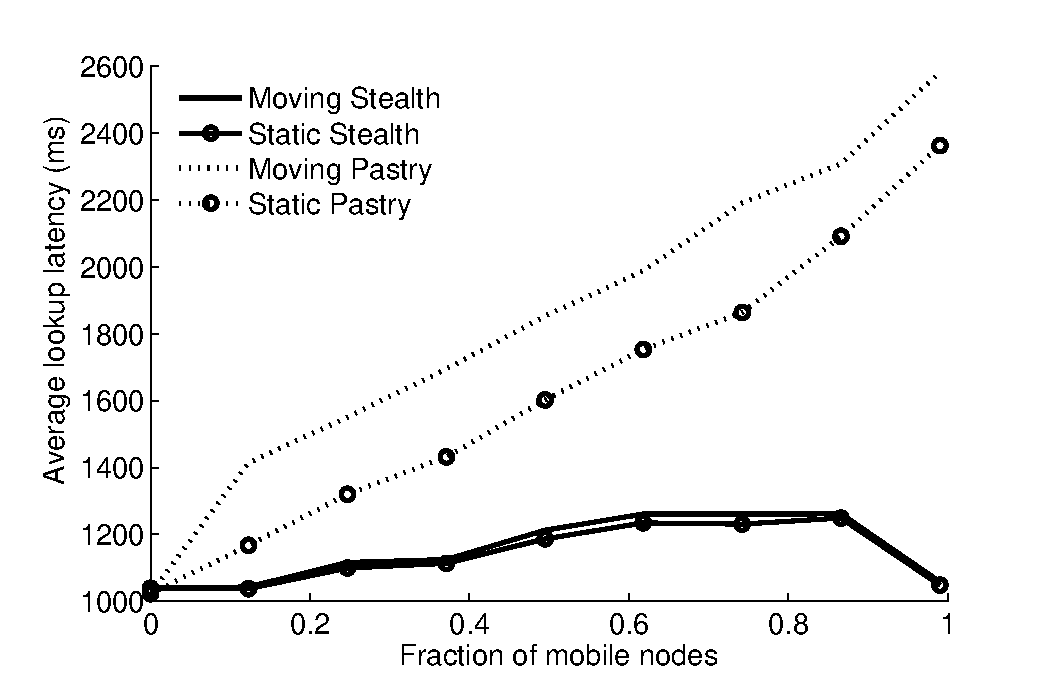
\epsfig{file= lookuplatency.eps, width=0.42\textwidth}
\caption{Average lookup latency} \label{fig:latency}
\end{figure}

Figure~\ref{fig:unreach}, however, shows a count of the number of
times a network packet was sent to a node which had since become
unreachable due to a change of address. Again, as stationary nodes
do not change IP address at any point, the points for the static
DHTs and also the first few for the moving DHTs (where the number of
wired nodes is high) are zero and thus not shown. It is important to
note that the figure shows results for all types of packet,
including those which are never resent (e.g. state messages, nodes
pinging one another and so on); this accounts for the discrepancy
between the number of unreachable destinations and the number of
resent messages. Unlike Figure~\ref{fig:rsnt}, results for the
moving Stealth DHT are displayed here; the reason for this is that
while service nodes are fixed, the stealth nodes making the requests
of them are not. As a result, a service node may attempt to reply
via IP to a stealth node, only to find that it is no longer
reachable. It is clear from this figure, however, that this
situation occurs far more often with Pastry than it does in a
Stealth DHT; the Stealth DHT does not even register any unreachable
nodes until 50\% of its stealth nodes are mobile.

\SubSection{Average lookup latency} \label{subsect:latency}

%We define {\em lookup latency} as the time elapsed between a node
%sending a {\em get} request into the DHT until the receipt of the
%corresponding {\em getreply} message. In addition to the effects of
%resending messages, the potentially low speed of wireless access and
%its propagation delay are some of the factors that can delay
%messages on a DHT.

Figure~\ref{fig:latency} shows the average {\em lookup latency}
(defined as the time elapsed between a node sending a {\em get}
request into the DHT until the receipt of the corresponding {\em
getreply} message) as a function of the fraction of mobile nodes for
moving and static Stealth and Pastry DHTs. The figure shows that
static and moving Stealth DHTs have similar end-to-end performance,
which is less than 1,300 ms for all considered networks. This shows
that Stealth DHTs maintain efficient routing performance independent
of the number of mobile nodes on the network.  The figure also shows
longer average latency for Pastry than for Stealth DHTs, as well as
the discrepancy increasing with the number of mobile nodes. We also
observe that moving Pastry suffers from longer average latency than
static Pastry. The figure shows that the maximum average latency
under Pastry is about twice the maximum value for Stealth DHTs. This
is to be expected, as the number of nodes performing forwarding
operations is lower in the Stealth DHT (1\% service nodes),
resulting in fewer hops on average.

In general, the figure shows quite  high average delays even for
Stealth DHTs (around 1.2 seconds). This is primarily due to the high
propagation delays of their access links (approximately 200ms each).

%\Section{Related Work}
%\label{sect-related}
%
%Hsiao {\em et al.}~\cite{towardsmobile} proposed a time-out free
%mobile DHT design, wherein stale state information and the
%associated maintenance overhead is reduced by allowing mobile nodes
%to invalidate information concerning themselves before moving. As it
%is not always possible for a node to know precisely when it will
%move, the invalidation of state information is accomplished by using
%periodic failure detection and recovery mechanisms already existing
%in most DHTs. In addition to these techniques, the paper discussed
%how other enhancements could be made, such as co-operative failure
%mechanisms and nodes discovering who their reverse neighbors are
%({\em i.e.} those who store information about them). The time-out
%free mobile DHT increases the state information required stored by
%nodes, as well as the signalling overhead for state maintenance. In
%practice, it seems that too much signalling overhead is required to
%quickly remove the node that is about to move.
%
%Hsiao {\em et al.}~\cite{mobilechurn} further investigated the
%performance of DHTs in a mobile environment, attempting to answer
%the question of whether or not the rudimentary solutions for failure
%handling and state recovery inherent in DHTs can efficiently handle
%mobility churn. The paper presents an intensive investigation on the
%performance difference between a generic implementation and an ideal
%one (in which nodes may invalidate all references to it before
%moving, as discussed earlier). Through simulation results, the paper
%concludes that a generic DHT can, in fact, have fair performance (in
%terms of object location latency and routing efficiency) when the
%system is placed under tremendously high ordinary churn and/or a
%high routing request rate. However, the rudimentary DHT
%implementation often introduces large maintenance overheads to the
%system. It is interesting to note that when outlining possible
%mobile DHT designs, this paper suggested excluding mobile nodes from
%relaying messages to avoid the performance problems associated with
%mobile nodes. The Stealth DHT algorithm also aims to do just that.
%
%Some of the design goals postulated
%in~\cite{mobilep2p1}\cite{mobilep2p2} match that of our Stealth DHT
%system, in that they aim to allow a provider to a) participate in
%creation and control of the service, b) to offer value-added
%services, such as higher performance and security while c)
%maintaining the characteristic of direct and efficient peer-to-peer
%interaction between users. This work differs from our own in that it
%uses eDonkey2000~\cite{donkey}, which makes use of central index
%servers to provide file-sharing services. Stealth DHTs, on the other
%hand, are decentralized distributed hash tables which can be used
%for many higher level applications.
%
%A number of works have considered designing DHT algorithms for
%mobile ad-hoc networks (MANETs)~\cite{dhtmanet01}\cite{ekta}. Ad-hoc
%networks differ from the networks discussed in this paper because
%they do not rely on any fixed infrastructure to communicate. We
%speculate that Stealth DHTs could also be used in MANETs after being
%suitably modified to allow for promotion/demotion between service
%and stealth nodes. This is left for future work.

\Section{Conclusion} \label{conclusion}

Peer-to-peer networking may increasingly have to cater for
intrinsically underpowered and unreliable mobile clients. In the
case of a generic DHT, its routing infrastructure may consist of a
large number of mobile nodes, leaving it susceptible to the
detrimental effects of mobility churn. Stealth DHTs offer a solution
to this problem by allowing for the isolation of mobile nodes
connected to it in order to deny the ability to execute any
operations that involve relaying and forwarding messages on the DHT.
Mobile nodes on the Stealth DHT are stealth nodes, and those
remaining are classed as service nodes. To accomplish the goals of
the Stealth DHT concept, nodes do not keep any state information
about stealth nodes in their routing state tables.

Using simulations, we have studied the effect of mobility churn on
Stealth DHTs and compared the results to Pastry. The results show
that the Stealth DHT algorithm is comparatively much more efficient
in reducing overhead on the network, and that it also offers
significantly higher routing efficiency. As expected, the simulation
results show that the performance of Stealth DHTs are not affected
by an increase in the number of mobile nodes on the network. For
Pastry, the results show that its performance degrades dramatically
as the ratio of mobile nodes to stationary nodes on the network
increases.

\bibliographystyle{latex8}
\bibliography{MP2P_MacQuire_A}

\end{document}
